% Options for packages loaded elsewhere
\PassOptionsToPackage{unicode}{hyperref}
\PassOptionsToPackage{hyphens}{url}
%
\documentclass[
]{article}
\title{Class 11: Transcriptomics \& RNA-Seq Data Analysis}
\author{Divya Shetty (A15390408)}
\date{2/22/2022}

\usepackage{amsmath,amssymb}
\usepackage{lmodern}
\usepackage{iftex}
\ifPDFTeX
  \usepackage[T1]{fontenc}
  \usepackage[utf8]{inputenc}
  \usepackage{textcomp} % provide euro and other symbols
\else % if luatex or xetex
  \usepackage{unicode-math}
  \defaultfontfeatures{Scale=MatchLowercase}
  \defaultfontfeatures[\rmfamily]{Ligatures=TeX,Scale=1}
\fi
% Use upquote if available, for straight quotes in verbatim environments
\IfFileExists{upquote.sty}{\usepackage{upquote}}{}
\IfFileExists{microtype.sty}{% use microtype if available
  \usepackage[]{microtype}
  \UseMicrotypeSet[protrusion]{basicmath} % disable protrusion for tt fonts
}{}
\makeatletter
\@ifundefined{KOMAClassName}{% if non-KOMA class
  \IfFileExists{parskip.sty}{%
    \usepackage{parskip}
  }{% else
    \setlength{\parindent}{0pt}
    \setlength{\parskip}{6pt plus 2pt minus 1pt}}
}{% if KOMA class
  \KOMAoptions{parskip=half}}
\makeatother
\usepackage{xcolor}
\IfFileExists{xurl.sty}{\usepackage{xurl}}{} % add URL line breaks if available
\IfFileExists{bookmark.sty}{\usepackage{bookmark}}{\usepackage{hyperref}}
\hypersetup{
  pdftitle={Class 11: Transcriptomics \& RNA-Seq Data Analysis},
  pdfauthor={Divya Shetty (A15390408)},
  hidelinks,
  pdfcreator={LaTeX via pandoc}}
\urlstyle{same} % disable monospaced font for URLs
\usepackage[margin=1in]{geometry}
\usepackage{color}
\usepackage{fancyvrb}
\newcommand{\VerbBar}{|}
\newcommand{\VERB}{\Verb[commandchars=\\\{\}]}
\DefineVerbatimEnvironment{Highlighting}{Verbatim}{commandchars=\\\{\}}
% Add ',fontsize=\small' for more characters per line
\usepackage{framed}
\definecolor{shadecolor}{RGB}{248,248,248}
\newenvironment{Shaded}{\begin{snugshade}}{\end{snugshade}}
\newcommand{\AlertTok}[1]{\textcolor[rgb]{0.94,0.16,0.16}{#1}}
\newcommand{\AnnotationTok}[1]{\textcolor[rgb]{0.56,0.35,0.01}{\textbf{\textit{#1}}}}
\newcommand{\AttributeTok}[1]{\textcolor[rgb]{0.77,0.63,0.00}{#1}}
\newcommand{\BaseNTok}[1]{\textcolor[rgb]{0.00,0.00,0.81}{#1}}
\newcommand{\BuiltInTok}[1]{#1}
\newcommand{\CharTok}[1]{\textcolor[rgb]{0.31,0.60,0.02}{#1}}
\newcommand{\CommentTok}[1]{\textcolor[rgb]{0.56,0.35,0.01}{\textit{#1}}}
\newcommand{\CommentVarTok}[1]{\textcolor[rgb]{0.56,0.35,0.01}{\textbf{\textit{#1}}}}
\newcommand{\ConstantTok}[1]{\textcolor[rgb]{0.00,0.00,0.00}{#1}}
\newcommand{\ControlFlowTok}[1]{\textcolor[rgb]{0.13,0.29,0.53}{\textbf{#1}}}
\newcommand{\DataTypeTok}[1]{\textcolor[rgb]{0.13,0.29,0.53}{#1}}
\newcommand{\DecValTok}[1]{\textcolor[rgb]{0.00,0.00,0.81}{#1}}
\newcommand{\DocumentationTok}[1]{\textcolor[rgb]{0.56,0.35,0.01}{\textbf{\textit{#1}}}}
\newcommand{\ErrorTok}[1]{\textcolor[rgb]{0.64,0.00,0.00}{\textbf{#1}}}
\newcommand{\ExtensionTok}[1]{#1}
\newcommand{\FloatTok}[1]{\textcolor[rgb]{0.00,0.00,0.81}{#1}}
\newcommand{\FunctionTok}[1]{\textcolor[rgb]{0.00,0.00,0.00}{#1}}
\newcommand{\ImportTok}[1]{#1}
\newcommand{\InformationTok}[1]{\textcolor[rgb]{0.56,0.35,0.01}{\textbf{\textit{#1}}}}
\newcommand{\KeywordTok}[1]{\textcolor[rgb]{0.13,0.29,0.53}{\textbf{#1}}}
\newcommand{\NormalTok}[1]{#1}
\newcommand{\OperatorTok}[1]{\textcolor[rgb]{0.81,0.36,0.00}{\textbf{#1}}}
\newcommand{\OtherTok}[1]{\textcolor[rgb]{0.56,0.35,0.01}{#1}}
\newcommand{\PreprocessorTok}[1]{\textcolor[rgb]{0.56,0.35,0.01}{\textit{#1}}}
\newcommand{\RegionMarkerTok}[1]{#1}
\newcommand{\SpecialCharTok}[1]{\textcolor[rgb]{0.00,0.00,0.00}{#1}}
\newcommand{\SpecialStringTok}[1]{\textcolor[rgb]{0.31,0.60,0.02}{#1}}
\newcommand{\StringTok}[1]{\textcolor[rgb]{0.31,0.60,0.02}{#1}}
\newcommand{\VariableTok}[1]{\textcolor[rgb]{0.00,0.00,0.00}{#1}}
\newcommand{\VerbatimStringTok}[1]{\textcolor[rgb]{0.31,0.60,0.02}{#1}}
\newcommand{\WarningTok}[1]{\textcolor[rgb]{0.56,0.35,0.01}{\textbf{\textit{#1}}}}
\usepackage{graphicx}
\makeatletter
\def\maxwidth{\ifdim\Gin@nat@width>\linewidth\linewidth\else\Gin@nat@width\fi}
\def\maxheight{\ifdim\Gin@nat@height>\textheight\textheight\else\Gin@nat@height\fi}
\makeatother
% Scale images if necessary, so that they will not overflow the page
% margins by default, and it is still possible to overwrite the defaults
% using explicit options in \includegraphics[width, height, ...]{}
\setkeys{Gin}{width=\maxwidth,height=\maxheight,keepaspectratio}
% Set default figure placement to htbp
\makeatletter
\def\fps@figure{htbp}
\makeatother
\setlength{\emergencystretch}{3em} % prevent overfull lines
\providecommand{\tightlist}{%
  \setlength{\itemsep}{0pt}\setlength{\parskip}{0pt}}
\setcounter{secnumdepth}{-\maxdimen} % remove section numbering
\ifLuaTeX
  \usepackage{selnolig}  % disable illegal ligatures
\fi

\begin{document}
\maketitle

\hypertarget{bioconductor-deseq-set-up}{%
\section{Bioconductor \& DESeq Set-up}\label{bioconductor-deseq-set-up}}

Install the necessary packages! Code below input into \emph{R console}.

\begin{Shaded}
\begin{Highlighting}[]
\CommentTok{\#install.packages("BiocManager")}
\CommentTok{\#BiocManager::install()}
\CommentTok{\#BiocManager::install("DESeq2")}
\end{Highlighting}
\end{Shaded}

Check that the packages were installed correctly.

\begin{Shaded}
\begin{Highlighting}[]
\FunctionTok{library}\NormalTok{(BiocManager)}
\FunctionTok{library}\NormalTok{(DESeq2)}
\end{Highlighting}
\end{Shaded}

\begin{verbatim}
## Loading required package: S4Vectors
\end{verbatim}

\begin{verbatim}
## Loading required package: stats4
\end{verbatim}

\begin{verbatim}
## Loading required package: BiocGenerics
\end{verbatim}

\begin{verbatim}
## 
## Attaching package: 'BiocGenerics'
\end{verbatim}

\begin{verbatim}
## The following objects are masked from 'package:stats':
## 
##     IQR, mad, sd, var, xtabs
\end{verbatim}

\begin{verbatim}
## The following objects are masked from 'package:base':
## 
##     anyDuplicated, append, as.data.frame, basename, cbind, colnames,
##     dirname, do.call, duplicated, eval, evalq, Filter, Find, get, grep,
##     grepl, intersect, is.unsorted, lapply, Map, mapply, match, mget,
##     order, paste, pmax, pmax.int, pmin, pmin.int, Position, rank,
##     rbind, Reduce, rownames, sapply, setdiff, sort, table, tapply,
##     union, unique, unsplit, which.max, which.min
\end{verbatim}

\begin{verbatim}
## 
## Attaching package: 'S4Vectors'
\end{verbatim}

\begin{verbatim}
## The following objects are masked from 'package:base':
## 
##     expand.grid, I, unname
\end{verbatim}

\begin{verbatim}
## Loading required package: IRanges
\end{verbatim}

\begin{verbatim}
## 
## Attaching package: 'IRanges'
\end{verbatim}

\begin{verbatim}
## The following object is masked from 'package:grDevices':
## 
##     windows
\end{verbatim}

\begin{verbatim}
## Loading required package: GenomicRanges
\end{verbatim}

\begin{verbatim}
## Loading required package: GenomeInfoDb
\end{verbatim}

\begin{verbatim}
## Loading required package: SummarizedExperiment
\end{verbatim}

\begin{verbatim}
## Loading required package: MatrixGenerics
\end{verbatim}

\begin{verbatim}
## Loading required package: matrixStats
\end{verbatim}

\begin{verbatim}
## 
## Attaching package: 'MatrixGenerics'
\end{verbatim}

\begin{verbatim}
## The following objects are masked from 'package:matrixStats':
## 
##     colAlls, colAnyNAs, colAnys, colAvgsPerRowSet, colCollapse,
##     colCounts, colCummaxs, colCummins, colCumprods, colCumsums,
##     colDiffs, colIQRDiffs, colIQRs, colLogSumExps, colMadDiffs,
##     colMads, colMaxs, colMeans2, colMedians, colMins, colOrderStats,
##     colProds, colQuantiles, colRanges, colRanks, colSdDiffs, colSds,
##     colSums2, colTabulates, colVarDiffs, colVars, colWeightedMads,
##     colWeightedMeans, colWeightedMedians, colWeightedSds,
##     colWeightedVars, rowAlls, rowAnyNAs, rowAnys, rowAvgsPerColSet,
##     rowCollapse, rowCounts, rowCummaxs, rowCummins, rowCumprods,
##     rowCumsums, rowDiffs, rowIQRDiffs, rowIQRs, rowLogSumExps,
##     rowMadDiffs, rowMads, rowMaxs, rowMeans2, rowMedians, rowMins,
##     rowOrderStats, rowProds, rowQuantiles, rowRanges, rowRanks,
##     rowSdDiffs, rowSds, rowSums2, rowTabulates, rowVarDiffs, rowVars,
##     rowWeightedMads, rowWeightedMeans, rowWeightedMedians,
##     rowWeightedSds, rowWeightedVars
\end{verbatim}

\begin{verbatim}
## Loading required package: Biobase
\end{verbatim}

\begin{verbatim}
## Welcome to Bioconductor
## 
##     Vignettes contain introductory material; view with
##     'browseVignettes()'. To cite Bioconductor, see
##     'citation("Biobase")', and for packages 'citation("pkgname")'.
\end{verbatim}

\begin{verbatim}
## 
## Attaching package: 'Biobase'
\end{verbatim}

\begin{verbatim}
## The following object is masked from 'package:MatrixGenerics':
## 
##     rowMedians
\end{verbatim}

\begin{verbatim}
## The following objects are masked from 'package:matrixStats':
## 
##     anyMissing, rowMedians
\end{verbatim}

\hypertarget{import-data}{%
\section{Import Data}\label{import-data}}

\begin{Shaded}
\begin{Highlighting}[]
\NormalTok{counts }\OtherTok{\textless{}{-}} \FunctionTok{read.csv}\NormalTok{(}\StringTok{"airway\_scaledcounts.csv"}\NormalTok{, }\AttributeTok{row.names =} \DecValTok{1}\NormalTok{)}
\NormalTok{metadata }\OtherTok{\textless{}{-}}  \FunctionTok{read.csv}\NormalTok{(}\StringTok{"airway\_metadata.csv"}\NormalTok{)}

\FunctionTok{head}\NormalTok{(counts)}
\end{Highlighting}
\end{Shaded}

\begin{verbatim}
##                 SRR1039508 SRR1039509 SRR1039512 SRR1039513 SRR1039516
## ENSG00000000003        723        486        904        445       1170
## ENSG00000000005          0          0          0          0          0
## ENSG00000000419        467        523        616        371        582
## ENSG00000000457        347        258        364        237        318
## ENSG00000000460         96         81         73         66        118
## ENSG00000000938          0          0          1          0          2
##                 SRR1039517 SRR1039520 SRR1039521
## ENSG00000000003       1097        806        604
## ENSG00000000005          0          0          0
## ENSG00000000419        781        417        509
## ENSG00000000457        447        330        324
## ENSG00000000460         94        102         74
## ENSG00000000938          0          0          0
\end{verbatim}

\begin{Shaded}
\begin{Highlighting}[]
\FunctionTok{head}\NormalTok{(metadata)}
\end{Highlighting}
\end{Shaded}

\begin{verbatim}
##           id     dex celltype     geo_id
## 1 SRR1039508 control   N61311 GSM1275862
## 2 SRR1039509 treated   N61311 GSM1275863
## 3 SRR1039512 control  N052611 GSM1275866
## 4 SRR1039513 treated  N052611 GSM1275867
## 5 SRR1039516 control  N080611 GSM1275870
## 6 SRR1039517 treated  N080611 GSM1275871
\end{verbatim}

\textbf{Q1. How many genes are in this dataset?}

\begin{Shaded}
\begin{Highlighting}[]
\FunctionTok{nrow}\NormalTok{(counts)}
\end{Highlighting}
\end{Shaded}

\begin{verbatim}
## [1] 38694
\end{verbatim}

There are 38694 genes.

\textbf{Q2. How many `control' cell lines do we have?}

\begin{Shaded}
\begin{Highlighting}[]
\FunctionTok{sum}\NormalTok{(metadata}\SpecialCharTok{$}\NormalTok{dex }\SpecialCharTok{==} \StringTok{"control"}\NormalTok{)}
\end{Highlighting}
\end{Shaded}

\begin{verbatim}
## [1] 4
\end{verbatim}

There are 4 `control' cell lines.

\hypertarget{differential-gene-expression-demo}{%
\section{Differential Gene Expression
DEMO}\label{differential-gene-expression-demo}}

Find the sample ID for the control cell lines, then calculate the mean
counts per gene for these samples.

\begin{Shaded}
\begin{Highlighting}[]
\NormalTok{control }\OtherTok{\textless{}{-}}\NormalTok{ metadata[metadata[,}\StringTok{"dex"}\NormalTok{] }\SpecialCharTok{==} \StringTok{"control"}\NormalTok{,]}
\NormalTok{control.counts }\OtherTok{\textless{}{-}}\NormalTok{ counts[ , control}\SpecialCharTok{$}\NormalTok{id]}
\NormalTok{control.mean }\OtherTok{\textless{}{-}} \FunctionTok{rowSums}\NormalTok{( control.counts ) }\SpecialCharTok{/} \DecValTok{4} 
\FunctionTok{head}\NormalTok{(control.mean)}
\end{Highlighting}
\end{Shaded}

\begin{verbatim}
## ENSG00000000003 ENSG00000000005 ENSG00000000419 ENSG00000000457 ENSG00000000460 
##          900.75            0.00          520.50          339.75           97.25 
## ENSG00000000938 
##            0.75
\end{verbatim}

The code below accomplishes the same task, except it uses the dplyr
package.

\begin{Shaded}
\begin{Highlighting}[]
\FunctionTok{library}\NormalTok{(dplyr)}
\end{Highlighting}
\end{Shaded}

\begin{verbatim}
## 
## Attaching package: 'dplyr'
\end{verbatim}

\begin{verbatim}
## The following object is masked from 'package:Biobase':
## 
##     combine
\end{verbatim}

\begin{verbatim}
## The following object is masked from 'package:matrixStats':
## 
##     count
\end{verbatim}

\begin{verbatim}
## The following objects are masked from 'package:GenomicRanges':
## 
##     intersect, setdiff, union
\end{verbatim}

\begin{verbatim}
## The following object is masked from 'package:GenomeInfoDb':
## 
##     intersect
\end{verbatim}

\begin{verbatim}
## The following objects are masked from 'package:IRanges':
## 
##     collapse, desc, intersect, setdiff, slice, union
\end{verbatim}

\begin{verbatim}
## The following objects are masked from 'package:S4Vectors':
## 
##     first, intersect, rename, setdiff, setequal, union
\end{verbatim}

\begin{verbatim}
## The following objects are masked from 'package:BiocGenerics':
## 
##     combine, intersect, setdiff, union
\end{verbatim}

\begin{verbatim}
## The following objects are masked from 'package:stats':
## 
##     filter, lag
\end{verbatim}

\begin{verbatim}
## The following objects are masked from 'package:base':
## 
##     intersect, setdiff, setequal, union
\end{verbatim}

\begin{Shaded}
\begin{Highlighting}[]
\NormalTok{control }\OtherTok{\textless{}{-}}\NormalTok{ metadata }\SpecialCharTok{\%\textgreater{}\%} \FunctionTok{filter}\NormalTok{(dex }\SpecialCharTok{==} \StringTok{"control"}\NormalTok{)}
\NormalTok{control.counts }\OtherTok{\textless{}{-}}\NormalTok{ counts }\SpecialCharTok{\%\textgreater{}\%} \FunctionTok{select}\NormalTok{(control}\SpecialCharTok{$}\NormalTok{id) }
\NormalTok{control.mean }\OtherTok{\textless{}{-}} \FunctionTok{rowSums}\NormalTok{(control.counts) }\SpecialCharTok{/} \DecValTok{4}
\FunctionTok{head}\NormalTok{(control.mean)}
\end{Highlighting}
\end{Shaded}

\begin{verbatim}
## ENSG00000000003 ENSG00000000005 ENSG00000000419 ENSG00000000457 ENSG00000000460 
##          900.75            0.00          520.50          339.75           97.25 
## ENSG00000000938 
##            0.75
\end{verbatim}

Using the dplyr package to accomplish this task is preferable because
the filtering of the data to identify the right samples is more
intuitive than the syntax from the previous example.

\textbf{Q3. How would you make the above code in either approach more
robust?}

I'd make the code more robust by changing the `4' to
`ncol(control.counts)' so that if the number of control samples were
changed, the mean would still be calculated accordingly. Refer below.

\begin{Shaded}
\begin{Highlighting}[]
\NormalTok{control.mean }\OtherTok{\textless{}{-}} \FunctionTok{rowSums}\NormalTok{(control.counts) }\SpecialCharTok{/} \FunctionTok{ncol}\NormalTok{(control.counts)}
\FunctionTok{head}\NormalTok{(control.mean)}
\end{Highlighting}
\end{Shaded}

\begin{verbatim}
## ENSG00000000003 ENSG00000000005 ENSG00000000419 ENSG00000000457 ENSG00000000460 
##          900.75            0.00          520.50          339.75           97.25 
## ENSG00000000938 
##            0.75
\end{verbatim}

\textbf{Q4. Follow the same procedure for the treated samples
(i.e.~calculate the mean per gene across drug treated samples and assign
to a labeled vector called treated.mean)}

\begin{Shaded}
\begin{Highlighting}[]
\NormalTok{treated }\OtherTok{\textless{}{-}}\NormalTok{ metadata }\SpecialCharTok{\%\textgreater{}\%} \FunctionTok{filter}\NormalTok{(dex }\SpecialCharTok{==} \StringTok{"treated"}\NormalTok{)}
\NormalTok{treated.counts }\OtherTok{\textless{}{-}}\NormalTok{ counts }\SpecialCharTok{\%\textgreater{}\%} \FunctionTok{select}\NormalTok{(treated}\SpecialCharTok{$}\NormalTok{id) }
\NormalTok{treated.mean }\OtherTok{\textless{}{-}} \FunctionTok{rowSums}\NormalTok{(treated.counts) }\SpecialCharTok{/} \FunctionTok{ncol}\NormalTok{(treated.counts)}
\FunctionTok{names}\NormalTok{(treated.mean) }\OtherTok{\textless{}{-}}\NormalTok{ counts}\SpecialCharTok{$}\NormalTok{ensgene}
\FunctionTok{head}\NormalTok{(treated.mean)}
\end{Highlighting}
\end{Shaded}

\begin{verbatim}
## [1] 658.00   0.00 546.00 316.50  78.75   0.00
\end{verbatim}

Comparing By raw counts is problematic, especially if we sequence one
group at a greater depth. A better approach would be to normalize by
sequencing depth per sample, which will be done later.

\begin{Shaded}
\begin{Highlighting}[]
\NormalTok{meancounts }\OtherTok{\textless{}{-}} \FunctionTok{data.frame}\NormalTok{(control.mean, treated.mean)}
\FunctionTok{colSums}\NormalTok{(meancounts)}
\end{Highlighting}
\end{Shaded}

\begin{verbatim}
## control.mean treated.mean 
##     23005324     22196524
\end{verbatim}

\textbf{Q5 (a). Create a scatter plot showing the mean of the treated
samples against the mean of the control samples.}

\begin{Shaded}
\begin{Highlighting}[]
\FunctionTok{plot}\NormalTok{(meancounts, }\AttributeTok{xlab =} \StringTok{"Control"}\NormalTok{, }\AttributeTok{ylab =} \StringTok{"Treated"}\NormalTok{)}
\end{Highlighting}
\end{Shaded}

\includegraphics{class11_files/figure-latex/plots-1.pdf}

\textbf{Q5 (b).You could also use the ggplot2 package to make this
figure producing the plot below. What geom\_?() function would you use
for this plot?}

You would use geom\_point().

\begin{Shaded}
\begin{Highlighting}[]
\FunctionTok{library}\NormalTok{(ggplot2)}
\FunctionTok{ggplot}\NormalTok{(meancounts) }\SpecialCharTok{+}
  \FunctionTok{aes}\NormalTok{(}\AttributeTok{x =}\NormalTok{ control.mean, }\AttributeTok{y =}\NormalTok{ treated.mean) }\SpecialCharTok{+} 
  \FunctionTok{geom\_point}\NormalTok{()}
\end{Highlighting}
\end{Shaded}

\includegraphics{class11_files/figure-latex/unnamed-chunk-11-1.pdf}

\textbf{Q6. Try plotting both axes on a log scale. What is the argument
to plot() that allows you to do this?}

For plot(), you can use the `log' argument. For ggplot(), you can use
`scale\_x\_continuous(trans = ``log2'')' and `scale\_y\_continuous(trans
= ``log2'')'.

\begin{Shaded}
\begin{Highlighting}[]
\FunctionTok{plot}\NormalTok{(meancounts, }\AttributeTok{xlab =} \StringTok{"Control"}\NormalTok{, }\AttributeTok{ylab =} \StringTok{"Treated"}\NormalTok{, }\AttributeTok{log =} \StringTok{"xy"}\NormalTok{)}
\end{Highlighting}
\end{Shaded}

\includegraphics{class11_files/figure-latex/unnamed-chunk-12-1.pdf}

Look for genes with large changes between control and treated samples
(use log2 of fold changes!). These can be candidate differentially
expressed genes.

\begin{Shaded}
\begin{Highlighting}[]
\NormalTok{meancounts}\SpecialCharTok{$}\NormalTok{log2fc }\OtherTok{\textless{}{-}} \FunctionTok{log2}\NormalTok{(meancounts[,}\StringTok{"treated.mean"}\NormalTok{] }\SpecialCharTok{/}\NormalTok{ meancounts[,}\StringTok{"control.mean"}\NormalTok{])}
\FunctionTok{head}\NormalTok{(meancounts)}
\end{Highlighting}
\end{Shaded}

\begin{verbatim}
##                 control.mean treated.mean      log2fc
## ENSG00000000003       900.75       658.00 -0.45303916
## ENSG00000000005         0.00         0.00         NaN
## ENSG00000000419       520.50       546.00  0.06900279
## ENSG00000000457       339.75       316.50 -0.10226805
## ENSG00000000460        97.25        78.75 -0.30441833
## ENSG00000000938         0.75         0.00        -Inf
\end{verbatim}

Find the genes that have unwanted values (ie. control.mean or untreated
mean being 0) and remove them from the results.

\begin{Shaded}
\begin{Highlighting}[]
\NormalTok{zero.vals }\OtherTok{\textless{}{-}} \FunctionTok{which}\NormalTok{(meancounts[,}\DecValTok{1}\SpecialCharTok{:}\DecValTok{2}\NormalTok{] }\SpecialCharTok{==} \DecValTok{0}\NormalTok{, }\AttributeTok{arr.ind =} \ConstantTok{TRUE}\NormalTok{)}

\NormalTok{to.rm }\OtherTok{\textless{}{-}} \FunctionTok{unique}\NormalTok{(zero.vals[,}\DecValTok{1}\NormalTok{])}
\NormalTok{mycounts }\OtherTok{\textless{}{-}}\NormalTok{ meancounts[}\SpecialCharTok{{-}}\NormalTok{to.rm,]}
\FunctionTok{head}\NormalTok{(mycounts)}
\end{Highlighting}
\end{Shaded}

\begin{verbatim}
##                 control.mean treated.mean      log2fc
## ENSG00000000003       900.75       658.00 -0.45303916
## ENSG00000000419       520.50       546.00  0.06900279
## ENSG00000000457       339.75       316.50 -0.10226805
## ENSG00000000460        97.25        78.75 -0.30441833
## ENSG00000000971      5219.00      6687.50  0.35769358
## ENSG00000001036      2327.00      1785.75 -0.38194109
\end{verbatim}

\textbf{Q7. What is the purpose of the arr.ind argument in the which()
function call above? Why would we then take the first column of the
output and need to call the unique() function?}

The arr.ind argument determines whether the which() function should
return the value of the index values. Setting it to TRUE means the
which() function above will return the indices of the row (gene) and
column (sample) where the conditions (control.mean == 0 or treated.mean
== 0) are met.

We want to remove the genes that have a 0 count, so we should remove the
rows that have a 0. As such, we use the first column of the output,
since this corresponds to the rows. We use the unique() function to make
sure we don't count a row (gene) twice,

Filter the dataset to see how many genes are up-regulated and
down-regulated!

\begin{Shaded}
\begin{Highlighting}[]
\NormalTok{up.ind }\OtherTok{\textless{}{-}}\NormalTok{ mycounts}\SpecialCharTok{$}\NormalTok{log2fc }\SpecialCharTok{\textgreater{}} \DecValTok{2}
\NormalTok{down.ind }\OtherTok{\textless{}{-}}\NormalTok{ mycounts}\SpecialCharTok{$}\NormalTok{log2fc }\SpecialCharTok{\textless{}}\NormalTok{ (}\SpecialCharTok{{-}}\DecValTok{2}\NormalTok{)}
\end{Highlighting}
\end{Shaded}

\textbf{Q8. Using the up.ind vector above can you determine how many up
regulated genes we have at the greater than 2 fc level?}

\begin{Shaded}
\begin{Highlighting}[]
\FunctionTok{sum}\NormalTok{(up.ind)}
\end{Highlighting}
\end{Shaded}

\begin{verbatim}
## [1] 250
\end{verbatim}

There are 250 up-regulated genes.

\textbf{Q9. Using the down.ind vector above can you determine how many
down regulated genes we have at the greater than 2 fc level?}

\begin{Shaded}
\begin{Highlighting}[]
\FunctionTok{sum}\NormalTok{(down.ind)}
\end{Highlighting}
\end{Shaded}

\begin{verbatim}
## [1] 367
\end{verbatim}

There are 367 down-regulated genes.

\textbf{Q10. Do you trust these results? Why or why not?}

No I don't trust these results because (1) these values were calculated
using raw counts, which as stated previously, doesn't consider sequence
depth and (2) the values weren't determined to be statistically
significant, meaning we don't know if these values actually indicate
differentially expressed genes.

\hypertarget{deseq-analysis}{%
\section{DESeq Analysis}\label{deseq-analysis}}

\begin{Shaded}
\begin{Highlighting}[]
\FunctionTok{citation}\NormalTok{(}\StringTok{"DESeq2"}\NormalTok{)}
\end{Highlighting}
\end{Shaded}

\begin{verbatim}
## 
##   Love, M.I., Huber, W., Anders, S. Moderated estimation of fold change
##   and dispersion for RNA-seq data with DESeq2 Genome Biology 15(12):550
##   (2014)
## 
## A BibTeX entry for LaTeX users is
## 
##   @Article{,
##     title = {Moderated estimation of fold change and dispersion for RNA-seq data with DESeq2},
##     author = {Michael I. Love and Wolfgang Huber and Simon Anders},
##     year = {2014},
##     journal = {Genome Biology},
##     doi = {10.1186/s13059-014-0550-8},
##     volume = {15},
##     issue = {12},
##     pages = {550},
##   }
\end{verbatim}

The DESeqDataSet is a single object that contains input values,
intermediate calculations like how things are normalized, and all
results of a differential expression analysis.

You can construct a DESeqDataSet from (1) a count matrix, (2) a metadata
file, and (3) a formula indicating the design of the experiment.

\begin{Shaded}
\begin{Highlighting}[]
\NormalTok{dds }\OtherTok{\textless{}{-}} \FunctionTok{DESeqDataSetFromMatrix}\NormalTok{(}\AttributeTok{countData =}\NormalTok{ counts, }
                              \AttributeTok{colData =}\NormalTok{ metadata, }
                              \AttributeTok{design=}\SpecialCharTok{\textasciitilde{}}\NormalTok{dex)}
\end{Highlighting}
\end{Shaded}

\begin{verbatim}
## converting counts to integer mode
\end{verbatim}

\begin{verbatim}
## Warning in DESeqDataSet(se, design = design, ignoreRank): some variables in
## design formula are characters, converting to factors
\end{verbatim}

\begin{Shaded}
\begin{Highlighting}[]
\NormalTok{dds}
\end{Highlighting}
\end{Shaded}

\begin{verbatim}
## class: DESeqDataSet 
## dim: 38694 8 
## metadata(1): version
## assays(1): counts
## rownames(38694): ENSG00000000003 ENSG00000000005 ... ENSG00000283120
##   ENSG00000283123
## rowData names(0):
## colnames(8): SRR1039508 SRR1039509 ... SRR1039520 SRR1039521
## colData names(4): id dex celltype geo_id
\end{verbatim}

Run the DESeq() on dds. This function calls a number of other functions
within the package to essentially run the entire DESeq pipeline. Extract
the results using results().

\begin{Shaded}
\begin{Highlighting}[]
\NormalTok{dds }\OtherTok{\textless{}{-}} \FunctionTok{DESeq}\NormalTok{(dds)}
\end{Highlighting}
\end{Shaded}

\begin{verbatim}
## estimating size factors
\end{verbatim}

\begin{verbatim}
## estimating dispersions
\end{verbatim}

\begin{verbatim}
## gene-wise dispersion estimates
\end{verbatim}

\begin{verbatim}
## mean-dispersion relationship
\end{verbatim}

\begin{verbatim}
## final dispersion estimates
\end{verbatim}

\begin{verbatim}
## fitting model and testing
\end{verbatim}

\begin{Shaded}
\begin{Highlighting}[]
\NormalTok{res }\OtherTok{\textless{}{-}} \FunctionTok{results}\NormalTok{(dds)}
\NormalTok{res}
\end{Highlighting}
\end{Shaded}

\begin{verbatim}
## log2 fold change (MLE): dex treated vs control 
## Wald test p-value: dex treated vs control 
## DataFrame with 38694 rows and 6 columns
##                  baseMean log2FoldChange     lfcSE      stat    pvalue
##                 <numeric>      <numeric> <numeric> <numeric> <numeric>
## ENSG00000000003  747.1942     -0.3507030  0.168246 -2.084470 0.0371175
## ENSG00000000005    0.0000             NA        NA        NA        NA
## ENSG00000000419  520.1342      0.2061078  0.101059  2.039475 0.0414026
## ENSG00000000457  322.6648      0.0245269  0.145145  0.168982 0.8658106
## ENSG00000000460   87.6826     -0.1471420  0.257007 -0.572521 0.5669691
## ...                   ...            ...       ...       ...       ...
## ENSG00000283115  0.000000             NA        NA        NA        NA
## ENSG00000283116  0.000000             NA        NA        NA        NA
## ENSG00000283119  0.000000             NA        NA        NA        NA
## ENSG00000283120  0.974916      -0.668258   1.69456 -0.394354  0.693319
## ENSG00000283123  0.000000             NA        NA        NA        NA
##                      padj
##                 <numeric>
## ENSG00000000003  0.163035
## ENSG00000000005        NA
## ENSG00000000419  0.176032
## ENSG00000000457  0.961694
## ENSG00000000460  0.815849
## ...                   ...
## ENSG00000283115        NA
## ENSG00000283116        NA
## ENSG00000283119        NA
## ENSG00000283120        NA
## ENSG00000283123        NA
\end{verbatim}

Convert res to a data frame and view the results.

\begin{Shaded}
\begin{Highlighting}[]
\NormalTok{res.df }\OtherTok{\textless{}{-}} \FunctionTok{as.data.frame}\NormalTok{(res)}
\FunctionTok{View}\NormalTok{(res.df)}
\end{Highlighting}
\end{Shaded}

The results function contains a number of arguments to customize the
results table. By default the argument alpha is set to 0.1. If the
adjusted p value cutoff will be a value other than 0.1, alpha should be
set to that value

\begin{Shaded}
\begin{Highlighting}[]
\NormalTok{res05 }\OtherTok{\textless{}{-}} \FunctionTok{results}\NormalTok{(dds, }\AttributeTok{alpha =} \FloatTok{0.05}\NormalTok{)}
\FunctionTok{summary}\NormalTok{(res05)}
\end{Highlighting}
\end{Shaded}

\begin{verbatim}
## 
## out of 25258 with nonzero total read count
## adjusted p-value < 0.05
## LFC > 0 (up)       : 1236, 4.9%
## LFC < 0 (down)     : 933, 3.7%
## outliers [1]       : 142, 0.56%
## low counts [2]     : 9033, 36%
## (mean count < 6)
## [1] see 'cooksCutoff' argument of ?results
## [2] see 'independentFiltering' argument of ?results
\end{verbatim}

\hypertarget{adding-annotation-data}{%
\section{Adding Annotation Data}\label{adding-annotation-data}}

Load annotation packages to help with mapping IDs between different
naming schemes.

\begin{Shaded}
\begin{Highlighting}[]
\FunctionTok{library}\NormalTok{(}\StringTok{"AnnotationDbi"}\NormalTok{)}
\end{Highlighting}
\end{Shaded}

\begin{verbatim}
## 
## Attaching package: 'AnnotationDbi'
\end{verbatim}

\begin{verbatim}
## The following object is masked from 'package:dplyr':
## 
##     select
\end{verbatim}

\begin{Shaded}
\begin{Highlighting}[]
\FunctionTok{library}\NormalTok{(}\StringTok{"org.Hs.eg.db"}\NormalTok{)}
\end{Highlighting}
\end{Shaded}

\begin{verbatim}
## 
\end{verbatim}

Below are all the avilable key types we could map between.

\begin{Shaded}
\begin{Highlighting}[]
\FunctionTok{columns}\NormalTok{(org.Hs.eg.db)}
\end{Highlighting}
\end{Shaded}

\begin{verbatim}
##  [1] "ACCNUM"       "ALIAS"        "ENSEMBL"      "ENSEMBLPROT"  "ENSEMBLTRANS"
##  [6] "ENTREZID"     "ENZYME"       "EVIDENCE"     "EVIDENCEALL"  "GENENAME"    
## [11] "GENETYPE"     "GO"           "GOALL"        "IPI"          "MAP"         
## [16] "OMIM"         "ONTOLOGY"     "ONTOLOGYALL"  "PATH"         "PFAM"        
## [21] "PMID"         "PROSITE"      "REFSEQ"       "SYMBOL"       "UCSCKG"      
## [26] "UNIPROT"
\end{verbatim}

We can use the mapIds() function to add individual columns to our
results table. We provide the row names of our results table as a key,
and specify that keytype=ENSEMBL. The column argument tells the mapIds()
function which information we want, and the multiVals argument tells the
function what to do if there are multiple possible values for a single
input value.

\begin{Shaded}
\begin{Highlighting}[]
\NormalTok{res}\SpecialCharTok{$}\NormalTok{symbol }\OtherTok{\textless{}{-}} \FunctionTok{mapIds}\NormalTok{(org.Hs.eg.db,}
                     \AttributeTok{keys =} \FunctionTok{row.names}\NormalTok{(res), }
                     \AttributeTok{keytype =} \StringTok{"ENSEMBL"}\NormalTok{,}
                     \AttributeTok{column =} \StringTok{"SYMBOL"}\NormalTok{,}
                     \AttributeTok{multiVals =} \StringTok{"first"}\NormalTok{)}
\end{Highlighting}
\end{Shaded}

\begin{verbatim}
## 'select()' returned 1:many mapping between keys and columns
\end{verbatim}

\begin{Shaded}
\begin{Highlighting}[]
\FunctionTok{head}\NormalTok{(res)}
\end{Highlighting}
\end{Shaded}

\begin{verbatim}
## log2 fold change (MLE): dex treated vs control 
## Wald test p-value: dex treated vs control 
## DataFrame with 6 rows and 7 columns
##                   baseMean log2FoldChange     lfcSE      stat    pvalue
##                  <numeric>      <numeric> <numeric> <numeric> <numeric>
## ENSG00000000003 747.194195     -0.3507030  0.168246 -2.084470 0.0371175
## ENSG00000000005   0.000000             NA        NA        NA        NA
## ENSG00000000419 520.134160      0.2061078  0.101059  2.039475 0.0414026
## ENSG00000000457 322.664844      0.0245269  0.145145  0.168982 0.8658106
## ENSG00000000460  87.682625     -0.1471420  0.257007 -0.572521 0.5669691
## ENSG00000000938   0.319167     -1.7322890  3.493601 -0.495846 0.6200029
##                      padj      symbol
##                 <numeric> <character>
## ENSG00000000003  0.163035      TSPAN6
## ENSG00000000005        NA        TNMD
## ENSG00000000419  0.176032        DPM1
## ENSG00000000457  0.961694       SCYL3
## ENSG00000000460  0.815849    C1orf112
## ENSG00000000938        NA         FGR
\end{verbatim}

\textbf{Q11. Run the mapIds() function three more times to add the
Entrez ID and UniProt accession and GENENAME as new columns called
res\(entrez, res\)uniprot and res\$genename.}

\begin{Shaded}
\begin{Highlighting}[]
\NormalTok{res}\SpecialCharTok{$}\NormalTok{entrez }\OtherTok{\textless{}{-}} \FunctionTok{mapIds}\NormalTok{(org.Hs.eg.db,}
                     \AttributeTok{keys =} \FunctionTok{row.names}\NormalTok{(res), }
                     \AttributeTok{keytype =} \StringTok{"ENSEMBL"}\NormalTok{,}
                     \AttributeTok{column =} \StringTok{"ENTREZID"}\NormalTok{,}
                     \AttributeTok{multiVals =} \StringTok{"first"}\NormalTok{)}
\end{Highlighting}
\end{Shaded}

\begin{verbatim}
## 'select()' returned 1:many mapping between keys and columns
\end{verbatim}

\begin{Shaded}
\begin{Highlighting}[]
\NormalTok{res}\SpecialCharTok{$}\NormalTok{uniprot }\OtherTok{\textless{}{-}} \FunctionTok{mapIds}\NormalTok{(org.Hs.eg.db,}
                     \AttributeTok{keys =} \FunctionTok{row.names}\NormalTok{(res), }
                     \AttributeTok{keytype =} \StringTok{"ENSEMBL"}\NormalTok{,}
                     \AttributeTok{column =} \StringTok{"UNIPROT"}\NormalTok{,}
                     \AttributeTok{multiVals =} \StringTok{"first"}\NormalTok{)}
\end{Highlighting}
\end{Shaded}

\begin{verbatim}
## 'select()' returned 1:many mapping between keys and columns
\end{verbatim}

\begin{Shaded}
\begin{Highlighting}[]
\NormalTok{res}\SpecialCharTok{$}\NormalTok{genename }\OtherTok{\textless{}{-}} \FunctionTok{mapIds}\NormalTok{(org.Hs.eg.db,}
                     \AttributeTok{keys =} \FunctionTok{row.names}\NormalTok{(res), }
                     \AttributeTok{keytype =} \StringTok{"ENSEMBL"}\NormalTok{,}
                     \AttributeTok{column =} \StringTok{"GENENAME"}\NormalTok{,}
                     \AttributeTok{multiVals =} \StringTok{"first"}\NormalTok{)}
\end{Highlighting}
\end{Shaded}

\begin{verbatim}
## 'select()' returned 1:many mapping between keys and columns
\end{verbatim}

\begin{Shaded}
\begin{Highlighting}[]
\FunctionTok{head}\NormalTok{(res)}
\end{Highlighting}
\end{Shaded}

\begin{verbatim}
## log2 fold change (MLE): dex treated vs control 
## Wald test p-value: dex treated vs control 
## DataFrame with 6 rows and 10 columns
##                   baseMean log2FoldChange     lfcSE      stat    pvalue
##                  <numeric>      <numeric> <numeric> <numeric> <numeric>
## ENSG00000000003 747.194195     -0.3507030  0.168246 -2.084470 0.0371175
## ENSG00000000005   0.000000             NA        NA        NA        NA
## ENSG00000000419 520.134160      0.2061078  0.101059  2.039475 0.0414026
## ENSG00000000457 322.664844      0.0245269  0.145145  0.168982 0.8658106
## ENSG00000000460  87.682625     -0.1471420  0.257007 -0.572521 0.5669691
## ENSG00000000938   0.319167     -1.7322890  3.493601 -0.495846 0.6200029
##                      padj      symbol      entrez     uniprot
##                 <numeric> <character> <character> <character>
## ENSG00000000003  0.163035      TSPAN6        7105  A0A024RCI0
## ENSG00000000005        NA        TNMD       64102      Q9H2S6
## ENSG00000000419  0.176032        DPM1        8813      O60762
## ENSG00000000457  0.961694       SCYL3       57147      Q8IZE3
## ENSG00000000460  0.815849    C1orf112       55732  A0A024R922
## ENSG00000000938        NA         FGR        2268      P09769
##                               genename
##                            <character>
## ENSG00000000003          tetraspanin 6
## ENSG00000000005            tenomodulin
## ENSG00000000419 dolichyl-phosphate m..
## ENSG00000000457 SCY1 like pseudokina..
## ENSG00000000460 chromosome 1 open re..
## ENSG00000000938 FGR proto-oncogene, ..
\end{verbatim}

Arrange and view by adjusted p-value!

\begin{Shaded}
\begin{Highlighting}[]
\NormalTok{ord }\OtherTok{\textless{}{-}} \FunctionTok{order}\NormalTok{(res}\SpecialCharTok{$}\NormalTok{padj)}
\FunctionTok{head}\NormalTok{(res[ord,])}
\end{Highlighting}
\end{Shaded}

\begin{verbatim}
## log2 fold change (MLE): dex treated vs control 
## Wald test p-value: dex treated vs control 
## DataFrame with 6 rows and 10 columns
##                  baseMean log2FoldChange     lfcSE      stat      pvalue
##                 <numeric>      <numeric> <numeric> <numeric>   <numeric>
## ENSG00000152583   954.771        4.36836 0.2371268   18.4220 8.74490e-76
## ENSG00000179094   743.253        2.86389 0.1755693   16.3120 8.10784e-60
## ENSG00000116584  2277.913       -1.03470 0.0650984  -15.8944 6.92855e-57
## ENSG00000189221  2383.754        3.34154 0.2124058   15.7319 9.14433e-56
## ENSG00000120129  3440.704        2.96521 0.2036951   14.5571 5.26424e-48
## ENSG00000148175 13493.920        1.42717 0.1003890   14.2164 7.25128e-46
##                        padj      symbol      entrez     uniprot
##                   <numeric> <character> <character> <character>
## ENSG00000152583 1.32441e-71     SPARCL1        8404  A0A024RDE1
## ENSG00000179094 6.13966e-56        PER1        5187      O15534
## ENSG00000116584 3.49776e-53     ARHGEF2        9181      Q92974
## ENSG00000189221 3.46227e-52        MAOA        4128      P21397
## ENSG00000120129 1.59454e-44       DUSP1        1843      B4DU40
## ENSG00000148175 1.83034e-42        STOM        2040      F8VSL7
##                               genename
##                            <character>
## ENSG00000152583           SPARC like 1
## ENSG00000179094 period circadian reg..
## ENSG00000116584 Rho/Rac guanine nucl..
## ENSG00000189221    monoamine oxidase A
## ENSG00000120129 dual specificity pho..
## ENSG00000148175               stomatin
\end{verbatim}

Write the ordered significant results with annotations.

\begin{Shaded}
\begin{Highlighting}[]
\FunctionTok{write.csv}\NormalTok{(res[ord,], }\StringTok{"deseq\_results1.csv"}\NormalTok{)}
\end{Highlighting}
\end{Shaded}

\hypertarget{data-visualization---volcano-plots}{%
\section{Data Visualization - Volcano
Plots}\label{data-visualization---volcano-plots}}

Volcano plots are used to highlight the proportion of genes that are
both significantly regulated and display a high fold change. Typically
these plots shows the log fold change on the X-axis, and the −log10 of
the p-value on the Y-axis.

\begin{Shaded}
\begin{Highlighting}[]
\FunctionTok{plot}\NormalTok{( res}\SpecialCharTok{$}\NormalTok{log2FoldChange,  }\SpecialCharTok{{-}}\FunctionTok{log}\NormalTok{(res}\SpecialCharTok{$}\NormalTok{padj), }
      \AttributeTok{xlab =} \StringTok{"Log2(FoldChange)"}\NormalTok{,}
      \AttributeTok{ylab =} \StringTok{"{-}Log(P{-}value)"}\NormalTok{)}
\end{Highlighting}
\end{Shaded}

\includegraphics{class11_files/figure-latex/unnamed-chunk-28-1.pdf}

Add cut off lines and color to make data visualization easier!

\begin{Shaded}
\begin{Highlighting}[]
\CommentTok{\#custom point color vector }
\NormalTok{mycols }\OtherTok{\textless{}{-}} \FunctionTok{rep}\NormalTok{(}\StringTok{"gray"}\NormalTok{, }\FunctionTok{nrow}\NormalTok{(res))}
\NormalTok{mycols[ }\FunctionTok{abs}\NormalTok{(res}\SpecialCharTok{$}\NormalTok{log2FoldChange) }\SpecialCharTok{\textgreater{}} \DecValTok{2}\NormalTok{ ]  }\OtherTok{\textless{}{-}} \StringTok{"red"} 

\NormalTok{inds }\OtherTok{\textless{}{-}}\NormalTok{ (res}\SpecialCharTok{$}\NormalTok{padj }\SpecialCharTok{\textless{}} \FloatTok{0.01}\NormalTok{) }\SpecialCharTok{\&}\NormalTok{ (}\FunctionTok{abs}\NormalTok{(res}\SpecialCharTok{$}\NormalTok{log2FoldChange) }\SpecialCharTok{\textgreater{}} \DecValTok{2}\NormalTok{ )}
\NormalTok{mycols[inds] }\OtherTok{\textless{}{-}} \StringTok{"blue"}

\CommentTok{\#plot with custom colors }
\FunctionTok{plot}\NormalTok{( res}\SpecialCharTok{$}\NormalTok{log2FoldChange,  }\SpecialCharTok{{-}}\FunctionTok{log}\NormalTok{(res}\SpecialCharTok{$}\NormalTok{padj), }
 \AttributeTok{col =}\NormalTok{ mycols, }\AttributeTok{ylab =} \StringTok{"{-}Log(P{-}value)"}\NormalTok{, }\AttributeTok{xlab =} \StringTok{"Log2(FoldChange)"}\NormalTok{ )}

\CommentTok{\#add cut{-}off lines}
\FunctionTok{abline}\NormalTok{(}\AttributeTok{v =} \FunctionTok{c}\NormalTok{(}\SpecialCharTok{{-}}\DecValTok{2}\NormalTok{,}\DecValTok{2}\NormalTok{), }\AttributeTok{col =} \StringTok{"darkgray"}\NormalTok{, }\AttributeTok{lty =} \DecValTok{2}\NormalTok{)}
\FunctionTok{abline}\NormalTok{(}\AttributeTok{h =} \SpecialCharTok{{-}}\FunctionTok{log}\NormalTok{(}\FloatTok{0.05}\NormalTok{), }\AttributeTok{col =} \StringTok{"darkgray"}\NormalTok{, }\AttributeTok{lty =} \DecValTok{2}\NormalTok{)}
\end{Highlighting}
\end{Shaded}

\includegraphics{class11_files/figure-latex/unnamed-chunk-29-1.pdf}

Use ENhanvedVolcano for more customization!

\begin{Shaded}
\begin{Highlighting}[]
\FunctionTok{library}\NormalTok{(EnhancedVolcano)}
\end{Highlighting}
\end{Shaded}

\begin{verbatim}
## Loading required package: ggrepel
\end{verbatim}

\begin{verbatim}
## Registered S3 methods overwritten by 'ggalt':
##   method                  from   
##   grid.draw.absoluteGrob  ggplot2
##   grobHeight.absoluteGrob ggplot2
##   grobWidth.absoluteGrob  ggplot2
##   grobX.absoluteGrob      ggplot2
##   grobY.absoluteGrob      ggplot2
\end{verbatim}

\begin{Shaded}
\begin{Highlighting}[]
\NormalTok{df }\OtherTok{\textless{}{-}} \FunctionTok{as.data.frame}\NormalTok{(res)}

\FunctionTok{EnhancedVolcano}\NormalTok{(df,}
    \AttributeTok{lab =}\NormalTok{ df}\SpecialCharTok{$}\NormalTok{symbol,}
    \AttributeTok{x =} \StringTok{\textquotesingle{}log2FoldChange\textquotesingle{}}\NormalTok{,}
    \AttributeTok{y =} \StringTok{\textquotesingle{}pvalue\textquotesingle{}}\NormalTok{)}
\end{Highlighting}
\end{Shaded}

\includegraphics{class11_files/figure-latex/unnamed-chunk-30-1.pdf}

\hypertarget{pathway-analysis}{%
\section{Pathway Analysis}\label{pathway-analysis}}

The KEGG pathway database, unlike GO for example, provides functional
annotation as well as information about gene products that interact with
each other in a given pathway, how they interact (e.g., activation,
inhibition, etc.), and where they interact (e.g., cytoplasm, nucleus,
etc.). Hence KEGG has the potential to provide extra insight beyond
annotation lists of simple molecular function, process etc. from GO
terms.

So set up the KEGG data sets needed!

\begin{Shaded}
\begin{Highlighting}[]
\FunctionTok{library}\NormalTok{(pathview)}
\end{Highlighting}
\end{Shaded}

\begin{verbatim}
## ##############################################################################
## Pathview is an open source software package distributed under GNU General
## Public License version 3 (GPLv3). Details of GPLv3 is available at
## http://www.gnu.org/licenses/gpl-3.0.html. Particullary, users are required to
## formally cite the original Pathview paper (not just mention it) in publications
## or products. For details, do citation("pathview") within R.
## 
## The pathview downloads and uses KEGG data. Non-academic uses may require a KEGG
## license agreement (details at http://www.kegg.jp/kegg/legal.html).
## ##############################################################################
\end{verbatim}

\begin{Shaded}
\begin{Highlighting}[]
\FunctionTok{library}\NormalTok{(gage)}
\end{Highlighting}
\end{Shaded}

\begin{verbatim}
## 
\end{verbatim}

\begin{Shaded}
\begin{Highlighting}[]
\FunctionTok{library}\NormalTok{(gageData)}

\FunctionTok{data}\NormalTok{(kegg.sets.hs)}

\CommentTok{\#examine the first 2 pathways in this kegg set for humans}
\FunctionTok{head}\NormalTok{(kegg.sets.hs, }\DecValTok{2}\NormalTok{)}
\end{Highlighting}
\end{Shaded}

\begin{verbatim}
## $`hsa00232 Caffeine metabolism`
## [1] "10"   "1544" "1548" "1549" "1553" "7498" "9"   
## 
## $`hsa00983 Drug metabolism - other enzymes`
##  [1] "10"     "1066"   "10720"  "10941"  "151531" "1548"   "1549"   "1551"  
##  [9] "1553"   "1576"   "1577"   "1806"   "1807"   "1890"   "221223" "2990"  
## [17] "3251"   "3614"   "3615"   "3704"   "51733"  "54490"  "54575"  "54576" 
## [25] "54577"  "54578"  "54579"  "54600"  "54657"  "54658"  "54659"  "54963" 
## [33] "574537" "64816"  "7083"   "7084"   "7172"   "7363"   "7364"   "7365"  
## [41] "7366"   "7367"   "7371"   "7372"   "7378"   "7498"   "79799"  "83549" 
## [49] "8824"   "8833"   "9"      "978"
\end{verbatim}

The main gage() function requires a named vector of fold changes, where
the names of the values are the Entrez gene IDs.

\begin{Shaded}
\begin{Highlighting}[]
\NormalTok{foldchanges }\OtherTok{=}\NormalTok{ res}\SpecialCharTok{$}\NormalTok{log2FoldChange}
\FunctionTok{names}\NormalTok{(foldchanges) }\OtherTok{=}\NormalTok{ res}\SpecialCharTok{$}\NormalTok{entrez}
\FunctionTok{head}\NormalTok{(foldchanges)}
\end{Highlighting}
\end{Shaded}

\begin{verbatim}
##        7105       64102        8813       57147       55732        2268 
## -0.35070302          NA  0.20610777  0.02452695 -0.14714205 -1.73228897
\end{verbatim}

Now run the gage pathway analysis!

\begin{Shaded}
\begin{Highlighting}[]
\NormalTok{keggres }\OtherTok{=} \FunctionTok{gage}\NormalTok{(foldchanges, }\AttributeTok{gsets=}\NormalTok{kegg.sets.hs)}
\end{Highlighting}
\end{Shaded}

\begin{Shaded}
\begin{Highlighting}[]
\FunctionTok{attributes}\NormalTok{(keggres)}
\end{Highlighting}
\end{Shaded}

\begin{verbatim}
## $names
## [1] "greater" "less"    "stats"
\end{verbatim}

\begin{Shaded}
\begin{Highlighting}[]
\CommentTok{\# Look at the first three down (less) pathways}
\FunctionTok{head}\NormalTok{(keggres}\SpecialCharTok{$}\NormalTok{less, }\DecValTok{3}\NormalTok{)}
\end{Highlighting}
\end{Shaded}

\begin{verbatim}
##                                       p.geomean stat.mean        p.val
## hsa05332 Graft-versus-host disease 0.0004250461 -3.473346 0.0004250461
## hsa04940 Type I diabetes mellitus  0.0017820293 -3.002352 0.0017820293
## hsa05310 Asthma                    0.0020045888 -3.009050 0.0020045888
##                                         q.val set.size         exp1
## hsa05332 Graft-versus-host disease 0.09053483       40 0.0004250461
## hsa04940 Type I diabetes mellitus  0.14232581       42 0.0017820293
## hsa05310 Asthma                    0.14232581       29 0.0020045888
\end{verbatim}

Now, let's try out the pathview() function to make a pathway plot with
our RNA-Seq expression results shown in color.

\begin{Shaded}
\begin{Highlighting}[]
\FunctionTok{pathview}\NormalTok{(}\AttributeTok{gene.data =}\NormalTok{ foldchanges, }\AttributeTok{pathway.id =} \StringTok{"hsa05310"}\NormalTok{)}
\end{Highlighting}
\end{Shaded}

\begin{verbatim}
## 'select()' returned 1:1 mapping between keys and columns
\end{verbatim}

\begin{verbatim}
## Info: Working in directory C:/Users/div/Documents/bimm143/labs/class11
\end{verbatim}

\begin{verbatim}
## Info: Writing image file hsa05310.pathview.png
\end{verbatim}

\begin{figure}
\centering
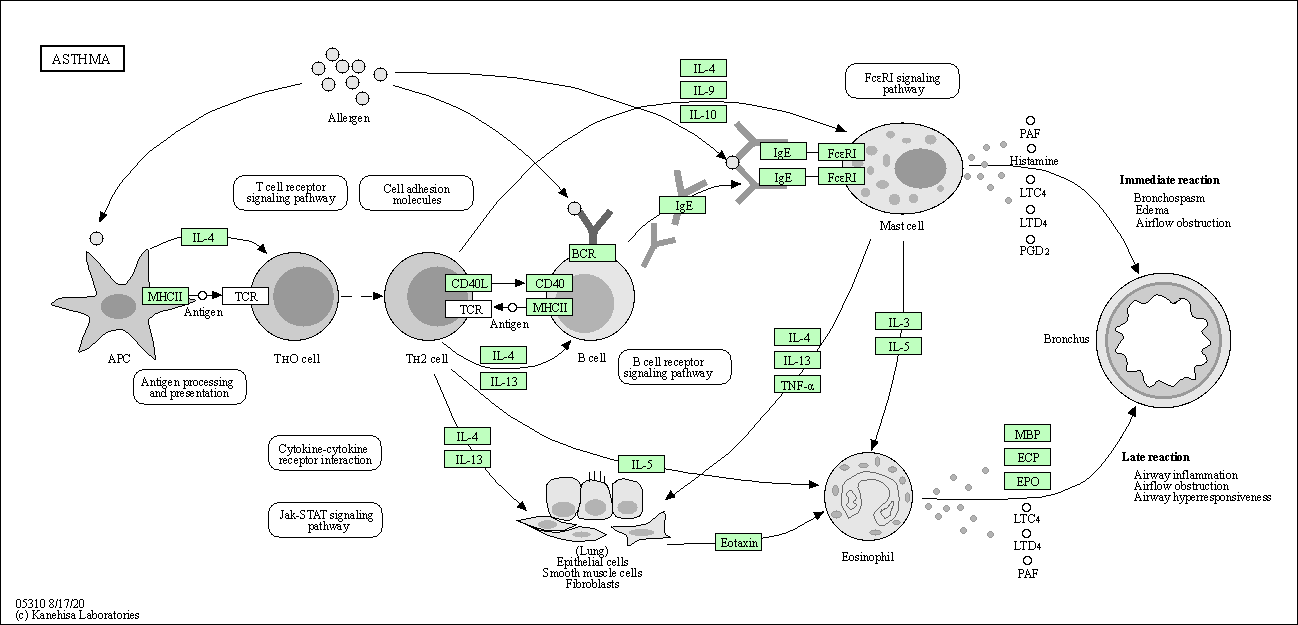
\includegraphics{hsa05310.png}
\caption{hsa05310 - Asthma}
\end{figure}

\textbf{Q12. Can you do the same procedure as above to plot the pathview
figures for the top 2 down-reguled pathways?}

\begin{Shaded}
\begin{Highlighting}[]
\FunctionTok{pathview}\NormalTok{(}\AttributeTok{gene.data =}\NormalTok{ foldchanges, }\AttributeTok{pathway.id =} \StringTok{"hsa05332"}\NormalTok{)}
\end{Highlighting}
\end{Shaded}

\begin{verbatim}
## 'select()' returned 1:1 mapping between keys and columns
\end{verbatim}

\begin{verbatim}
## Info: Working in directory C:/Users/div/Documents/bimm143/labs/class11
\end{verbatim}

\begin{verbatim}
## Info: Writing image file hsa05332.pathview.png
\end{verbatim}

\begin{Shaded}
\begin{Highlighting}[]
\FunctionTok{pathview}\NormalTok{(}\AttributeTok{gene.data =}\NormalTok{ foldchanges, }\AttributeTok{pathway.id =} \StringTok{"hsa04940"}\NormalTok{)}
\end{Highlighting}
\end{Shaded}

\begin{verbatim}
## 'select()' returned 1:1 mapping between keys and columns
\end{verbatim}

\begin{verbatim}
## Info: Working in directory C:/Users/div/Documents/bimm143/labs/class11
\end{verbatim}

\begin{verbatim}
## Info: Writing image file hsa04940.pathview.png
\end{verbatim}

\begin{figure}
\centering
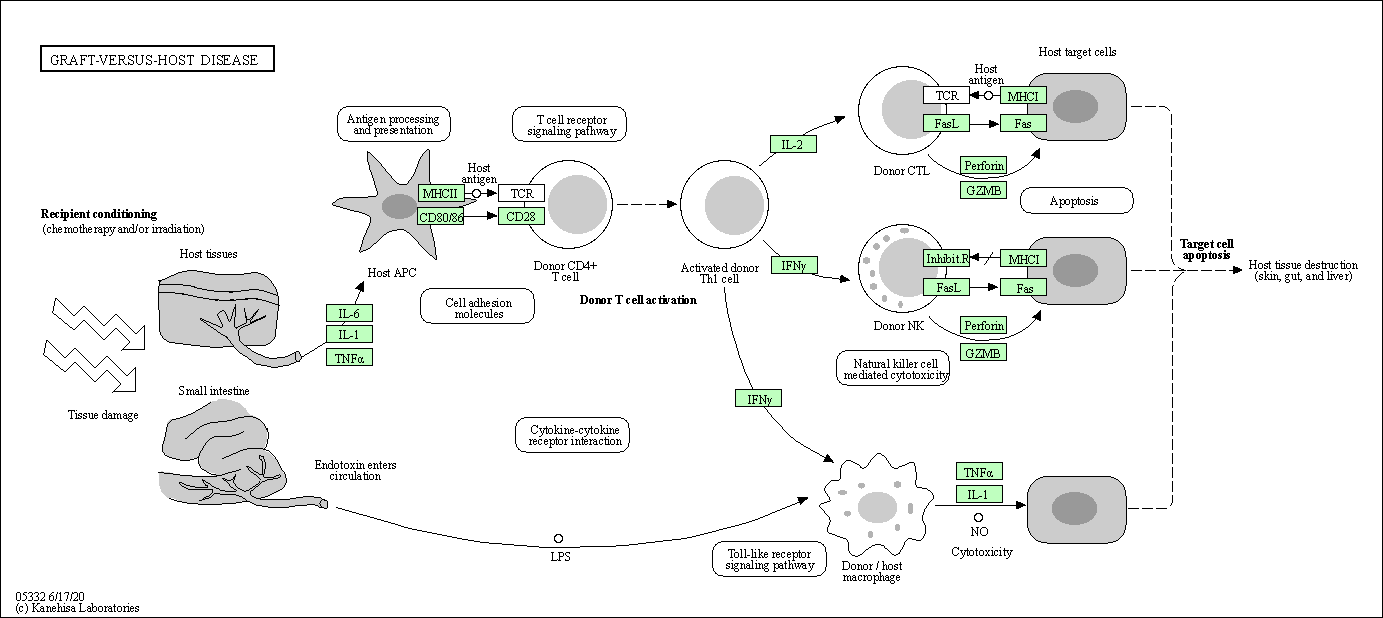
\includegraphics{hsa05332.png}
\caption{hsa05332}
\end{figure}

\begin{figure}
\centering
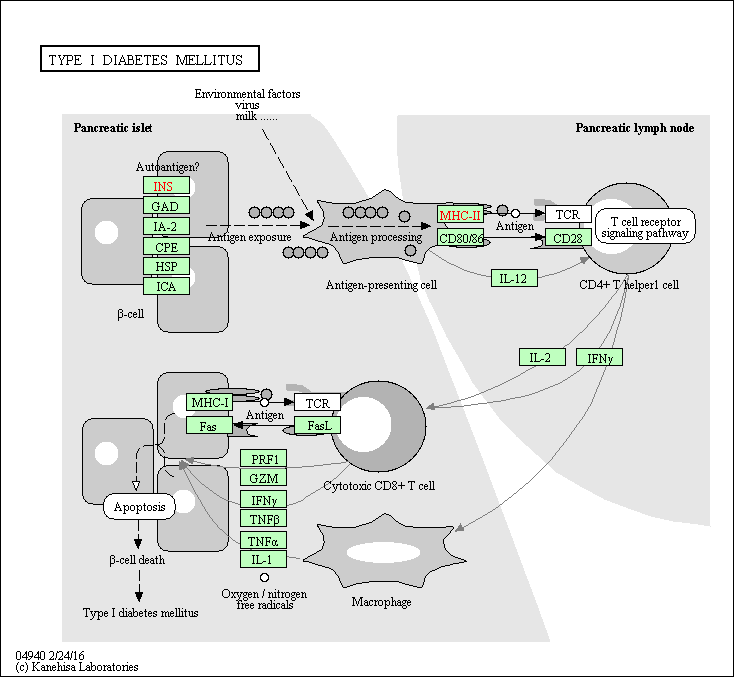
\includegraphics{hsa04940.png}
\caption{hsa04940}
\end{figure}

\hypertarget{plotting-counts-for-gene-of-interest}{%
\section{Plotting Counts for Gene of
Interest}\label{plotting-counts-for-gene-of-interest}}

First, find the gene ID for the CRISPLD2 genes.

\begin{Shaded}
\begin{Highlighting}[]
\NormalTok{i }\OtherTok{\textless{}{-}} \FunctionTok{grep}\NormalTok{(}\StringTok{"CRISPLD2"}\NormalTok{, res}\SpecialCharTok{$}\NormalTok{symbol)}
\NormalTok{res[i,]}
\end{Highlighting}
\end{Shaded}

\begin{verbatim}
## log2 fold change (MLE): dex treated vs control 
## Wald test p-value: dex treated vs control 
## DataFrame with 1 row and 10 columns
##                  baseMean log2FoldChange     lfcSE      stat      pvalue
##                 <numeric>      <numeric> <numeric> <numeric>   <numeric>
## ENSG00000103196   3096.16        2.62603  0.267444   9.81899 9.32747e-23
##                        padj      symbol      entrez     uniprot
##                   <numeric> <character> <character> <character>
## ENSG00000103196 3.36344e-20    CRISPLD2       83716  A0A140VK80
##                               genename
##                            <character>
## ENSG00000103196 cysteine rich secret..
\end{verbatim}

\begin{Shaded}
\begin{Highlighting}[]
\FunctionTok{rownames}\NormalTok{(res[i,])}
\end{Highlighting}
\end{Shaded}

\begin{verbatim}
## [1] "ENSG00000103196"
\end{verbatim}

Now plot the counts! plotCounts() takes a DESeqDataSet that has been run
through the pipeline, the name of a gene, and the name of the variable
in the colData that you're interested in, and plots those values.

\begin{Shaded}
\begin{Highlighting}[]
\FunctionTok{plotCounts}\NormalTok{(dds, }\AttributeTok{gene =} \StringTok{"ENSG00000103196"}\NormalTok{, }\AttributeTok{intgroup =} \StringTok{"dex"}\NormalTok{)}
\end{Highlighting}
\end{Shaded}

\includegraphics{class11_files/figure-latex/unnamed-chunk-39-1.pdf}

Returns the counts as a data frame.

\begin{Shaded}
\begin{Highlighting}[]
\NormalTok{d }\OtherTok{\textless{}{-}} \FunctionTok{plotCounts}\NormalTok{(dds, }\AttributeTok{gene =} \StringTok{"ENSG00000103196"}\NormalTok{, }\AttributeTok{intgroup =} \StringTok{"dex"}\NormalTok{, }\AttributeTok{returnData =} \ConstantTok{TRUE}\NormalTok{)}
\end{Highlighting}
\end{Shaded}

Now we can make a boxplot and ggplot of the data.

\begin{Shaded}
\begin{Highlighting}[]
\FunctionTok{boxplot}\NormalTok{(count }\SpecialCharTok{\textasciitilde{}}\NormalTok{ dex , }\AttributeTok{data =}\NormalTok{ d)}
\end{Highlighting}
\end{Shaded}

\includegraphics{class11_files/figure-latex/unnamed-chunk-41-1.pdf}

\begin{Shaded}
\begin{Highlighting}[]
\FunctionTok{ggplot}\NormalTok{(d, }\FunctionTok{aes}\NormalTok{(dex, count, }\AttributeTok{fill =}\NormalTok{ dex)) }\SpecialCharTok{+} 
  \FunctionTok{geom\_boxplot}\NormalTok{() }\SpecialCharTok{+} 
  \FunctionTok{scale\_y\_log10}\NormalTok{() }\SpecialCharTok{+} 
  \FunctionTok{ggtitle}\NormalTok{(}\StringTok{"CRISPLD2"}\NormalTok{)}
\end{Highlighting}
\end{Shaded}

\includegraphics{class11_files/figure-latex/unnamed-chunk-41-2.pdf}

\end{document}
